\documentclass[twoside, fontsize=11pt, chapterprefix=false]{scrbook}

% For dummy text only
\usepackage{blindtext}

% For PDF document without binding offset
\usepackage[a4paper, bindingoffset=0cm,left=2.5cm, right=2.5cm, top=2.5cm, bottom=2.5cm]{geometry}

% Print (with binding offset)
%\usepackage[a4paper, bindingoffset=0.3cm,left=2.5cm, right=2.2cm, top=2.5cm, bottom=3cm]{geometry}

% Textwidth is 6.3 inches (Size your figures accordingly)
\usepackage{titlesec}
\usepackage{color}
\usepackage{colortbl}
\definecolor{darkblue}{RGB}{50,107,164} % Bootstrap style
%\definecolor{darkblue}{RGB}{0,0,0} % Bootstrap style
\usepackage{pdfpages}

\usepackage[usenames,dvipsnames]{xcolor}
\usepackage[helvetica]{quotchap}
\usepackage{gensymb}
\usepackage{xspace}

% Nicer fonts
\usepackage[sfdefault]{roboto}
%\usepackage[T1]{fontenc}
\usepackage{charter}
\usepackage[bitstream-charter]{mathdesign}
\renewcommand{\familydefault}{\rmdefault}

% Set font for description env
\usepackage{enumitem}
\setlist[description]{%
  topsep=25pt,               % space before start / after end of list
  itemsep=5pt,               % space between items
  font={\normalfont\bfseries}  % set the label font
}


\usepackage{layouts}
\usepackage[utf8]{inputenc}
\usepackage{textcomp}
\usepackage{multirow}
\usepackage[english]{babel}
\usepackage{ngerman}
\usepackage{longtable} 
%\usepackage{amsmath}
%\usepackage{amssymb}
\usepackage{graphicx}
\usepackage{epstopdf}
%\usepackage{array}
\usepackage{booktabs}
%\usepackage{paralist}
%\usepackage{calc}
%\usepackage{nomencl}
\usepackage{tabulary}
%\usepackage{tabularx}
\usepackage{url}
\urlstyle{same}

\usepackage{float}
\usepackage[hang, bf]{caption}
\usepackage{subcaption}
\captionsetup{width=0.9\textwidth}

%
\usepackage{fancyhdr}

% Handling of floats
\usepackage[section,verbose]{placeins}
\usepackage[all]{nowidow}

% Alter some LaTeX defaults for better treatment of figures:
    % See p.105 of "TeX Unbound" for suggested values.
    % See pp. 199-200 of Lamport's "LaTeX" book for details.
    %   General parameters, for ALL pages:
    \renewcommand{\topfraction}{0.9}	% max fraction of floats at top
    \renewcommand{\bottomfraction}{0.8}	% max fraction of floats at bottom
    %   Parameters for TEXT pages (not float pages):
    \setcounter{topnumber}{2}
    \setcounter{bottomnumber}{2}
    \setcounter{totalnumber}{4}     % 2 may work better
    \setcounter{dbltopnumber}{2}    % for 2-column pages
    \renewcommand{\dbltopfraction}{0.9}	% fit big float above 2-col. text
    \renewcommand{\textfraction}{0.07}	% allow minimal text w. figs
    %   Parameters for FLOAT pages (not text pages):
    \renewcommand{\floatpagefraction}{0.7}	% require fuller float pages
	% N.B.: floatpagefraction MUST be less than topfraction !!
    \renewcommand{\dblfloatpagefraction}{0.7}	% require fuller float pages

%selbst installierte packages
\usepackage{natbib}
\usepackage{bibentry}
\nobibliography*

% % Für Druckversion % % Auch binding offset einstellen!!!
%\definecolor{darkblue}{RGB}{0,0,0} % Bootstrap style
%\makeatletter
%\def\NAT@nmfmt#1{\textit{#1}}
%\makeatother

% Counts
\usepackage{totcount}
\newtotcounter{citenum}
\def\oldcite{}
\let\oldcite=\bibcite
\def\bibcite{\stepcounter{citenum}\oldcite}
\usepackage[figure,table]{totalcount}

%\usepackage[percent]{overpic}
%\usepackage{wallpaper}
%\usepackage{rotating}
%\usepackage{units}

%\usepackage{microtype}
%itemize
\renewcommand{\labelitemi}{$\bullet$}
\renewcommand{\labelitemii}{$\circ$}
\renewcommand{\labelitemiii}{$\cdot$}
\renewcommand{\labelitemiv}{$\ast$}

\selectlanguage{english}

\setlength{\parindent}{0pt}
\setlength{\parskip}{8pt}     % Absatzabstand

\usepackage{lastpage}
\usepackage[pdfpagelabels=true,plainpages=false, linktoc=all]{hyperref}
\usepackage{bookmark}
\usepackage{afterpage}

\makeatletter
\newcommand*\Autoref[1]{%
  \begingroup
    \let\ORI@HyRef@testreftype\HyRef@testreftype
    \def\HyRef@testreftype##1.##2\\{%
      \ORI@HyRef@testreftype##1.##2\\%
      \let\ORI@HyRef@currentHtag\HyRef@currentHtag
      \def\HyRef@currentHtag{\expandafter\MakeUppercase}%
      \expandafter\g@addto@macro\expandafter\HyRef@currentHtag\expandafter{\ORI@HyRef@currentHtag}%
    }%
    \autoref{#1}%
  \endgroup}
\makeatother
\hypersetup{
    plainpages=false,
    bookmarks=true,         % show bookmarks bar?
    unicode=false,          % non-Latin characters in Acrobat's bookmarks
    pdftoolbar=true,        % show Acrobat's toolbar?
    pdfmenubar=true,        % show Acrobat's menu?
    pdffitwindow=true,      % page fit to window when opened    ´
    pdftitle={PhD thesis, Florian M. Wagner, ETH Zurich (2016)},    % title
    pdfauthor={Florian Michael Wagner},     % author
    pdfsubject={New developments in electrical resistivity imaging with applications to geological CO\textsubscript{2} storage},   % subject of the document
    pdfnewwindow=true,      % links in new window
    pdfkeywords={Carbon dioxide storage, Electrical resistivity monitoring, Experimental design, Borehole effects, Hydrogeophysical inversion}, % list of keywords
    colorlinks=true,       % false: boxed links; true: colored links
    linkcolor=darkblue,    % color of internal links
    citecolor=darkblue,        % color of links to bibliography
    filecolor=darkblue,      % color of file links
    urlcolor=darkblue,           % color of external links
    bookmarksnumbered=true, %Lesezeichen werden nummeriert dargestellt
    pdfdisplaydoctitle=true,
    pdfstartview=FitV,
    linktocpage=true,
%    pdfpagelayout = {TwoPageRight},
}

% Line spacing
\renewcommand{\baselinestretch}{1.50}\normalsize
\setlength{\headheight}{1.1\baselineskip}
\def\sectionautorefname{Section}

% Smaller linespacing in figure captions
\usepackage{setspace}
\captionsetup{font={small, stretch=1.2}}

\newcommand{\co}{CO\textsubscript{2}\xspace}

% Chapter headings
\makeatletter
\renewcommand*{\sectfont}{\bfseries}
\renewcommand*{\chapnumfont}{%
  \usefont{T1}{\@defaultcnfont}{b}{n}\fontsize{100}{120}\selectfont% Default: 100/130
  \color{chaptergrey}%
}
\makeatother

% Signature and Date snippet
\newcommand*{\SignatureAndDate}[1]{%
    \par\noindent\makebox[2.5in]{\hrulefill} \hfill\makebox[2.0in]{\hrulefill}%
    \par\noindent\makebox[2.5in][l]{#1}      \hfill\makebox[2.0in][l]{Date}%
}%

%\usepackage{pifont} % checkboxes

\usepackage[breakable, theorems, skins]{tcolorbox}
\tcbset{enhanced}

\definecolor{lightgrey}{HTML}{F5F5F5}
%\definecolor{lightgrey}{gray}{0.95}
\definecolor{darkgrey}{gray}{0.92}
\definecolor{rulegrey}{gray}{0.82}

\DeclareRobustCommand{\mybox}[2][lightgrey]{%
\begin{tcolorbox}[   %% Adjust the following parameters at will.
        breakable,
        left=5pt,
        right=5pt,
        top=5pt,
        bottom=5pt,
        colback=#1,
        colframe=darkgrey,
        width=\dimexpr\textwidth\relax, 
        enlarge left by=0mm,
        boxsep=5pt,
        arc=5pt,outer arc=5pt,
        ]
        #2
\end{tcolorbox}
}

\newcommand{\cref}[1]{\Autoref{#1} (\nameref{#1})}

\renewcommand{\autodot}{}% Remove all end-of-counter dots

\usepackage{etoolbox}

% Show or do not show A,B,C in pdf bookmarks
\providecommand*\texorpdfstring[2]{#1}
\providecommand*\appendixmore{}% falls appendixprefix=false
\newcommand*{\SavedOriginalchaptertocentry}{}
\appto\appendixmore{%
  \let\SavedOriginaladdchaptertocentry\addchaptertocentry
  \renewcommand*{\addchaptertocentry}[2]{%
    \ifstr{#1}{}{
      \SavedOriginalchaptertocentry{#1}{#2}
    }
    {
      \SavedOriginaladdchaptertocentry{}{%
        \texorpdfstring{
          \string\expandafter\string\MakeUppercase\string\appendixname
          ~#1:\string\enskip{}#2
        }{#2}%
      }%
    }%
  }%
}

% References
\newlength{\bibitemsep}\setlength{\bibitemsep}{.2\baselineskip plus .05\baselineskip minus .05\baselineskip}
\newlength{\bibparskip}\setlength{\bibparskip}{0pt}
\let\oldthebibliography\thebibliography
\renewcommand\thebibliography[1]{%
  \oldthebibliography{#1}%
  \setlength{\parskip}{\bibitemsep}%
  \setlength{\itemsep}{\bibparskip}%
}

% for CV
\definecolor{lightgray}{gray}{0.8}
\newcolumntype{F}{>{\raggedleft}p{0.14\textwidth}}
\newcolumntype{W}{p{0.8\textwidth}}
\newcommand\VRule{\color{lightgray}\vrule width 0.5pt}

% HEADER
\pagestyle{fancy}
\fancypagestyle{main}{%
  \fancyhf{}%
  \renewcommand{\headrulewidth}{2.5pt}% 2pt header rule
  \renewcommand{\headrule}{\hbox to\headwidth{%
  \color{rulegrey}\leaders\hrule height \headrulewidth\hfill}}
  \fancyhead[EC]{\sffamily\nouppercase\leftmark}
  \fancyhead[OC]{\sffamily\nouppercase\rightmark}
  \fancyhead[EL]{\sffamily\bfseries\textbf\thepage}
  \fancyhead[OR]{\sffamily\bfseries\textbf\thepage}
  \fancyheadoffset{0cm}
}
\fancypagestyle{plain}{%
  \fancyhf{}%
  \renewcommand{\headrulewidth}{0pt}% 2pt header rule
  \fancyfoot[EL]{\bfseries\thepage} % bei druck auskommentieren
  \fancyfoot[OR]{\bfseries\thepage}
}

\appto\frontmatter{\pagestyle{empty}}
\appto\mainmatter{\pagestyle{main}}
\appto\backmatter{\pagestyle{main}}

\usepackage{minitoc}

% Folder to figures of each chapter
\graphicspath{
{./2_exp_design/}
{./3_borehole_effects/}
{./4_hydrogeophysical_inversion/}
{./appendix/brine_migration/}
{./appendix/ketzin_ert/}
{./appendix/ketzin_review/}
{./appendix/long_term_aspects/}
}

\begin{document}
\dominitoc
\pagestyle{empty}    % switch to "empty" page style for front matter of document
%%Titelblatt
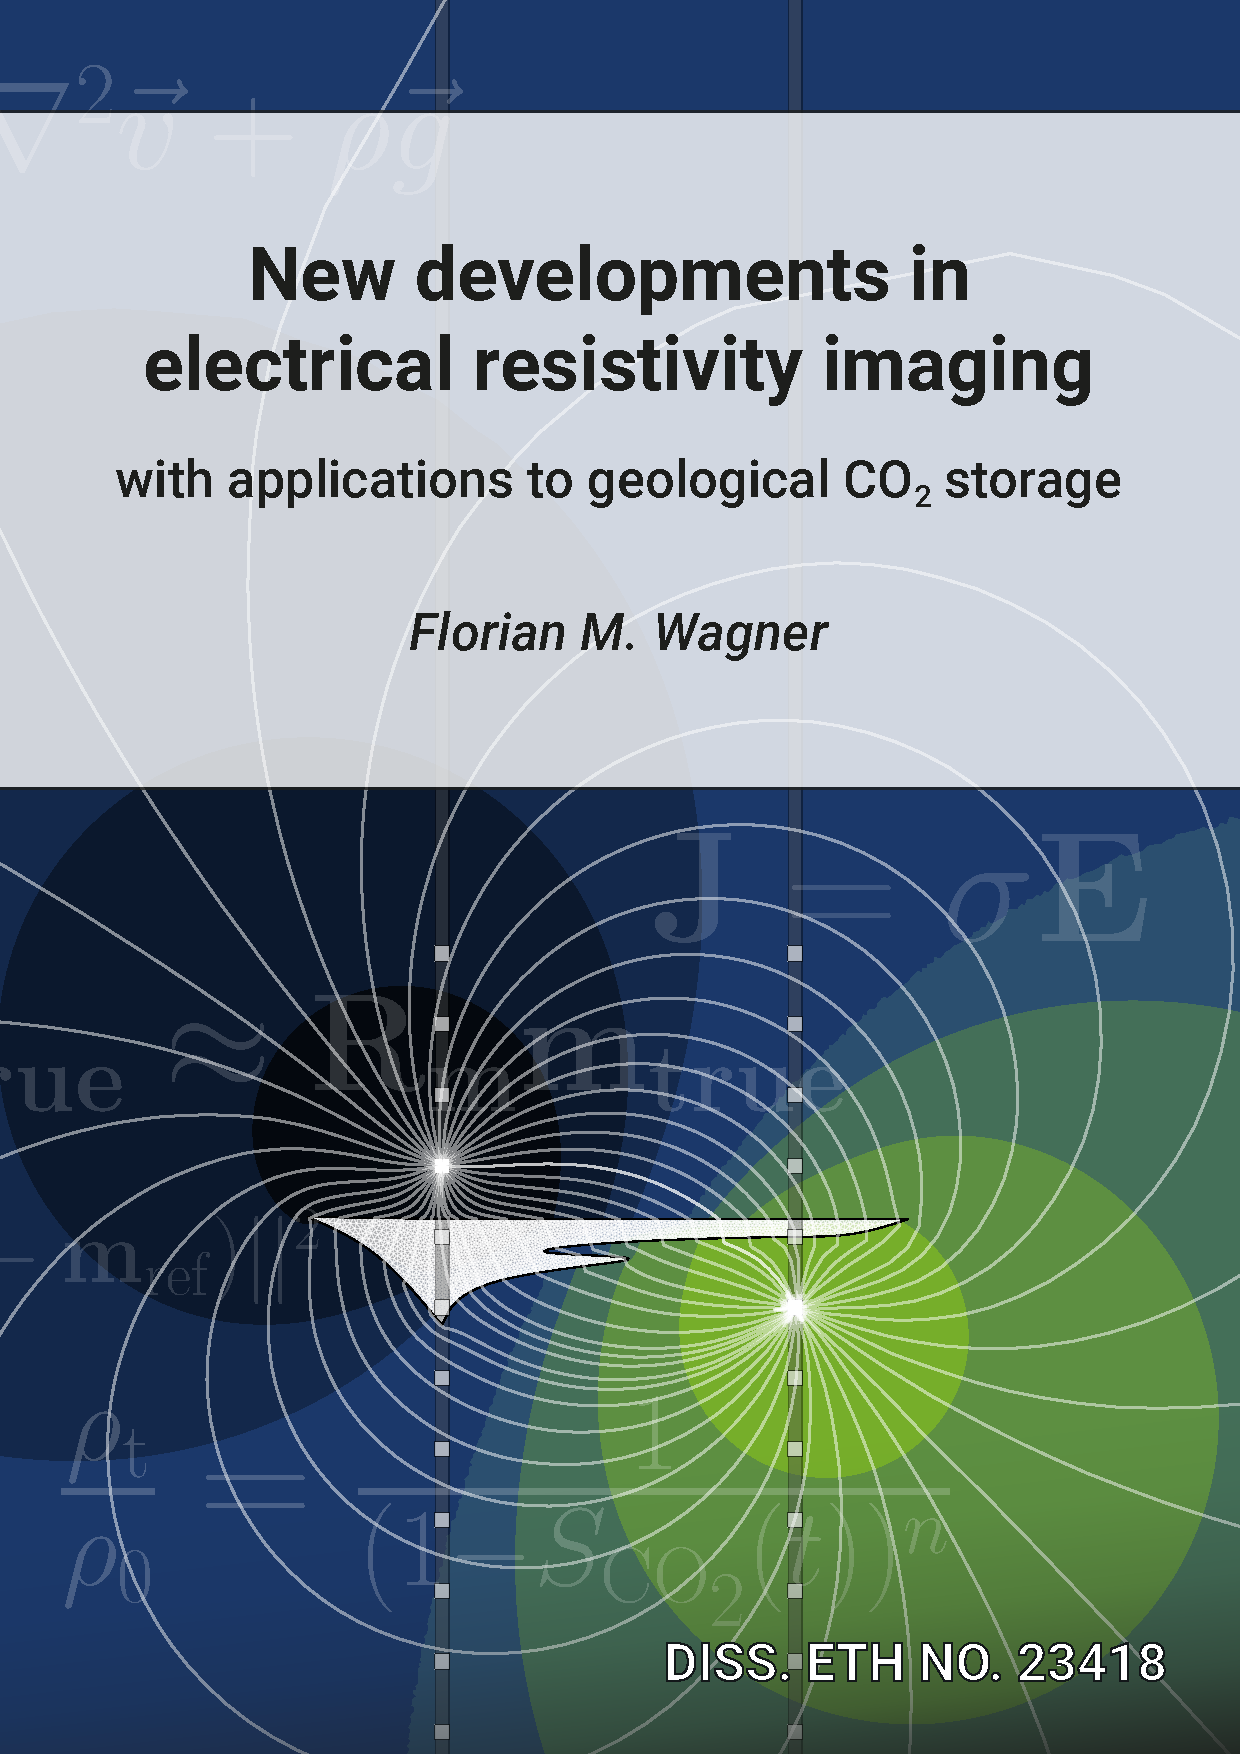
\includepdf[fitpaper]{front.pdf} %\cleardoubleemptypage

% DISSERTATION FRONT PAGE
% ----------------------------------------------------------------
\begin{titlepage}
\begin{center}
{\large
DISS. ETH NO. 23418\\
}
%\vfill
\vspace{1cm}
{\LARGE
%\bfseries\textsc{New developments in electrical resistivity imaging\\with applications to geological \co storage} \\[0.5cm]
\Large\bfseries{NEW DEVELOPMENTS IN ELECTRICAL RESISTIVITY IMAGING\\WITH APPLICATIONS TO GEOLOGICAL CO\textsubscript{2} STORAGE} \\[0.5cm]
}
\vfill
{\large
%A thesis submitted to\\
A thesis submitted to attain the degree of\\
\vspace{0.1cm}
DOCTOR OF SCIENCES of ETH ZURICH\\
%\vspace{0.1cm}
%ETH ZURICH\\
%\vspace{0.1cm}
%to attain the degree of\\
%\vspace{0.1cm}
%DOCTOR OF SCIENCES\\
\vspace{0.1cm}
(Dr. sc. ETH Zurich)\\
\vspace{0.4cm}
\vfill
presented by\\
\vspace{0.5cm}
\textbf{Florian Michael Wagner}\\
\vspace{0.5cm}
{\itshape
M.Sc. Applied Geophysics\\
TU Delft, ETH Zurich, RWTH Aachen University\\}
\vspace{0.25cm}
born on May 8, 1987\\
citizen of Germany\\
\vfill
accepted on the recommendation of\\[0.5cm] %should be changed to accepted!!


Prof. Dr. Hansruedi Maurer, examiner\\
Dr. Cornelia Schmidt-Hattenberger, co-examiner\\
Prof. Dr. Martin O. Saar, co-examiner\\
Prof. Dr. Andrew Binley, co-examiner\\
}
\vfill
{\large
2016\\}
\vfill
%(222 pages, \totalfigures{} figures, \totaltables{} tables, and \total{citenum} references)
\end{center}

\end{titlepage}
 %\newpage
\renewcommand\chapterheadstartvskip{\vspace*{-1\baselineskip}}

% % % % % % % % % % % % % % % % % % % % % % % % % % % % % % % %
\vspace*{\fill}
\mybox{\large
\textbf{Abstract and fulltext available under:}\\
Wagner, Florian Michael. New developments in electrical resistivity imaging with applications to geological \co storage. ETH-Z\"urich (2016). \url{http://dx.doi.org/10.3929/ethz-a-010636965}.

%(222 pages, \totalfigures{} figures, \totaltables{} tables, and \total{citenum} references)
}
%\chapter*{Abstract}
\blindtext
\cleardoubleemptypage

%\pdfbookmark[chapter]{Kurzfassung}{Kurzfassung}
\chapter*{Kurzfassung}
\selectlanguage{ngerman}
\blindtext
\selectlanguage{english}


\cleardoubleemptypage
% % % % % % % % % % % % % % % % % % % % % % % % % % % % % % % %

\frontmatter
\pagenumbering{Roman}

\pagestyle{plain}
\renewcommand\chapterheadstartvskip{}


% ABSTRACT
\pdfbookmark[chapter]{Abstract}{Abstract}
\chapter*{Abstract}
\blindtext
\cleardoubleemptypage

%\pdfbookmark[chapter]{Kurzfassung}{Kurzfassung}
\chapter*{Kurzfassung}
\selectlanguage{ngerman}
\blindtext
\selectlanguage{english}\cleardoubleemptypage

% ACKNOWLEDGEMENTS
\pdfbookmark[chapter]{Acknowledgments}{Acknowledgments}
\chapter*{Acknowledgments}
\setlength{\parskip}{0.68em}
\setlength{\parindent}{0em}


% Consider leaving this
I thank Florian Wagner for making the \LaTeX\,template of this thesis available at \url{https://github.com/florian-wagner/thesis-tex-template}.
\setlength{\parindent}{0pt}
\setlength{\parskip}{8pt}

\cleardoubleemptypage

% TABLE OF CONTENTS
\setcounter{tocdepth}{1} % Only subsections?
\pdfbookmark[chapter]{\contentsname}{toc}
\tableofcontents\cleardoubleemptypage

% LIST OF FIGURES
%\listoffigures
%\addcontentsline{toc}{chapter}{List of Figures}

% LIST OF TABLES
%\listoftables
%\addcontentsline{toc}{chapter}{List of Tables}

% MAIN CONTENT
% Section title font styles

\titleformat{\section}[hang]{\usefont{T1}{qhv}{b}{n}\selectfont}
{\Large\thesection}{13pt}{\Large}[{\titlerule[0pt]}]

\titleformat{\section}
{\sffamily\Large\bfseries}{\thesection}{0.8em}{}
\titleformat{\subsection}
{\sffamily\bfseries\large}{\thesubsection}{0.8em}{}
\titleformat{\subsubsection}
{\sffamily\bfseries\normalsize}{\thesubsubsection}{0.8em}{}
\titleformat{\paragraph}[runin]
{\sffamily\bfseries\normalsize}{\theparagraph}{0.8em}{}
\titleformat{\subparagraph}[runin]
{\sffamily\bfseries\normalsize}{\thesubparagraph}{1em}{}

\titlespacing\section{0pt}{11pt plus 4pt minus 2pt}{0pt plus 2pt minus 2pt}
\titlespacing\subsection{0pt}{11pt plus 4pt minus 2pt}{0pt plus 2pt minus 2pt}
\titlespacing\subsubsection{0pt}{11pt plus 4pt minus 2pt}{0pt plus 2pt minus 2pt}
\titlespacing\paragraph{0pt}{11pt plus 4pt minus 2pt}{0pt plus 2pt minus 2pt}
\titlespacing\subparagraph{0pt}{11pt plus 4pt minus 2pt}{0pt plus 2pt minus 2pt}

\setcounter{mtc}{0}
\mainmatter
\chapter{Introduction}\label{chap:theory}
\minitoc
\vfill
\mybox{
	This chapter gives an introduction to the geological storage of carbon dioxide, geoelectrical monitoring, and the studied field site.
	Finally, the research objectives and structure of this thesis are outlined.
	The given introduction aims to provide a basis for the individual papers comprised in this cumulative thesis and does not attempt to represent a general overview.
}

\section{Geological \co storage}

\subsection{Motivation and potential}
\citep{Archie1942}
\Blindtext



\begin{figure}[htbp]
	\centering
	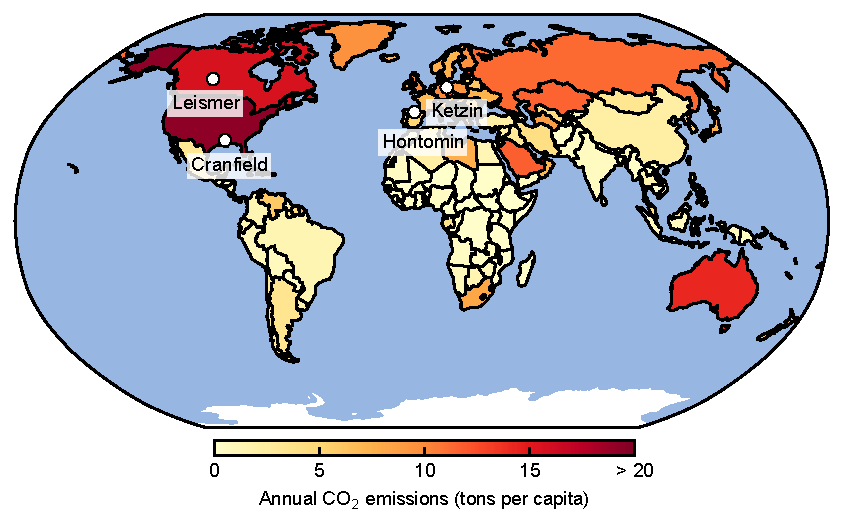
\includegraphics[width=.9\textwidth]{figs/map.pdf}
	\caption{Overview of deep permanent electrode installations. The map is colored by annual \co emissions in metric tons per capita averaged between 1960 and 2015 \citep{Bank2015}.}
	\label{fig:map}
\end{figure}
%

\cref{chap:theory} introduces the underlying inversion theory as used in the code by \cite{Ruecker2017}.
\cleardoubleemptypage
\chapter{Theory}\label{chap:theory}
\minitoc
\vfill
\mybox{
	This chapter introduces the underlying mathematics.
}

\section{Linear inversion}

\blindmathtrue
\blindmathpaper

\section{Non-linear Inversion}\cleardoubleemptypage
\blinddocument
\blinddocument

% INCLUDE OTHER CHAPTER HERE


%% APENDIX
\phantomsection
\addcontentsline{toc}{part}{Appendices}
%\pdfbookmark[part]{Appendices}{Appendices}
\part*{Appendices}\label{dissappendix}\cleardoubleemptypage
\begin{appendix}
%\fancypagestyle{plain}{%
%  \fancyhf{}%
%  \renewcommand{\headrulewidth}{0pt}% 2pt header rule
%  %\fancyfoot[EL]{\textbf\thepage}
%  \fancyfoot[OR]{\textbf\thepage}
%}
% INCLUDE APPENDICES HERE
%\include{./appendix/ketzin_review/ketzin_review}\cleardoubleemptypage
\end{appendix}

\backmatter
\renewcommand\chapterheadstartvskip{}
\patchcmd{\bibsetup}{\interlinepenalty=5000}{\interlinepenalty=10000}{}{} % avoid page break in bibtex
\bookmarksetup{startatroot}
\begingroup
    \setlength{\bibhang}{10mm}
    \bibliographystyle{copernicus}
    \renewcommand\bibname{References}
    \small
    \setlength{\bibsep}{11pt}
    \setstretch{1.15}
    \bibliography{references}
\endgroup

\addcontentsline{toc}{chapter}{References}
\addtocontents{toc}{
\protect\enlargethispage{\baselineskip}
}
\cleardoubleemptypage

\setstretch{1.1}
\pagestyle{plain}
\renewcommand{\headrulewidth}{0pt}
\chapter{Curriculum Vitae}
\titlespacing\section{0pt}{11pt plus 4pt minus 2pt}{11pt plus 4pt minus 2pt}
\section*{Personal}
\begin{tabular}{F!{\VRule}W}
Full Name & -\\[5pt]
Date of Birth & -\\[5pt]
Place of Birth & -\\[5pt]
Citizenship & -\\[5pt]
Website & -
\end{tabular}

\section*{Education}
\begin{tabular}{F!{\VRule}W}
2006\,--\,2009&-\\[5pt]
2009\,--\,2011&-\\[5pt]
2012\,--\,2016&-
\end{tabular}

\section*{Professional Experience}
\begin{tabular}{F!{\VRule}W}
Mar. 2009-\\[5pt]
July 2010&-\\[5pt]
Sept. 2013&-\\[5pt]
Nov. 2011\\-- May 2016&-
\end{tabular}
\clearpage
\mbox{}
\thispagestyle{empty}

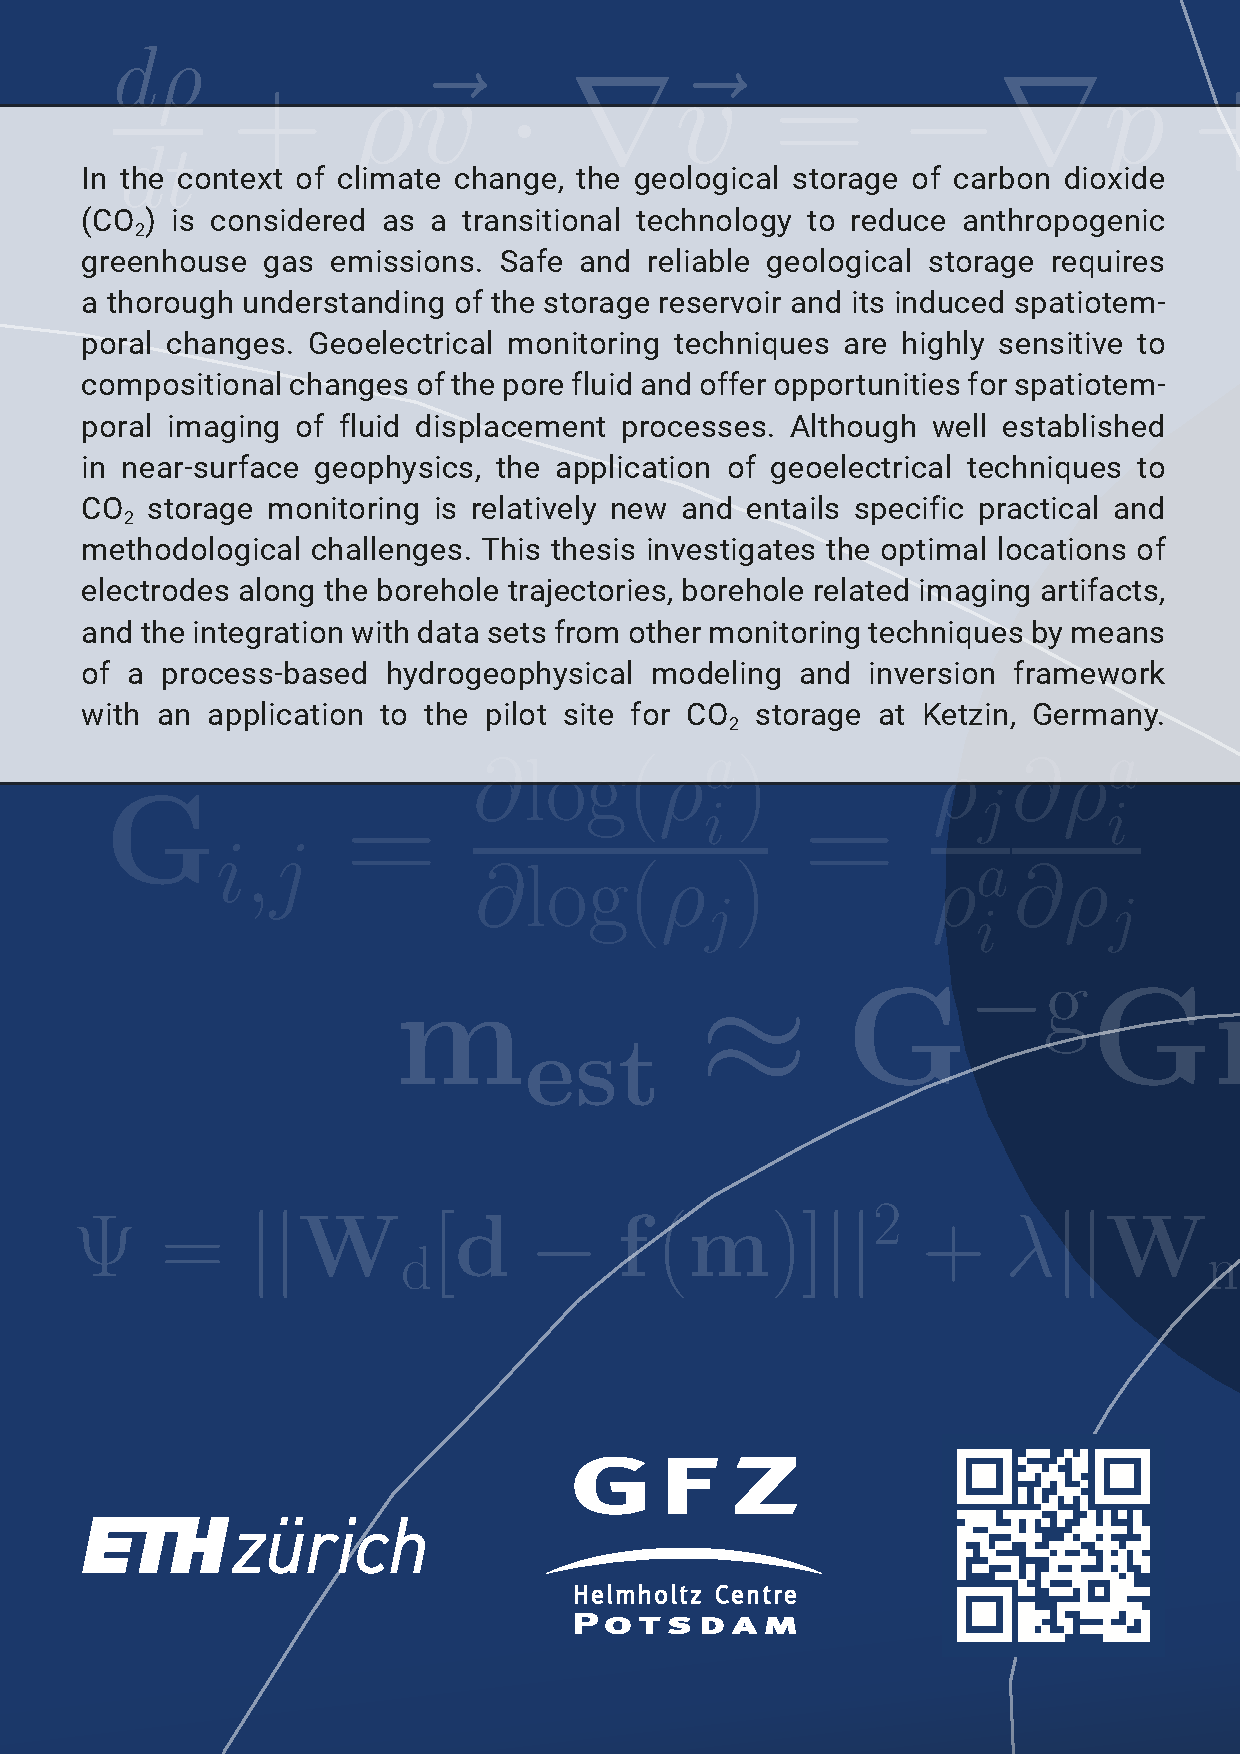
\includepdf[fitpaper]{back}
\end{document}
